\chapter{Introduction: The Bias Against Exploration Misallocates Creative Attention}

On problem-solving, Albert Einstein said, ``\textit{If I had an hour to solve a problem I’d spend 55 minutes thinking about the problem and 5 minutes thinking about solutions.}’’ Yet a common bias in problem-solving is under-allocating up front effort and attention to exploration because exploring a path not taken feels like a waste of time. Why even contemplate a red chair if you know that ‘of course’ the chair will be blue in the end? The problem with not exploring the possibility of the chair being red is that we neglect the possibility that the red chair might inspire us to do something different with the blue chair, that we will actually prefer the red chair, or that the red chair might be a stepping stone to another unconsidered option altogether. When we lock ourselves into believing that one solution is the only solution, we get stuck on individual ‘trees’ rather than seeing the full ‘forest.’

\section{Creative Thinking as Annealing}

Creative problems are complex; they consist of multiple possible approaches and solutions. Like simulated annealing, creative thinking starts with a “hot” exploratory phase of searching broadly and then gradually “cools” to an exploitation phase of searching narrowly and refining ideas \cite{kirkpatrick1983optimization, lucas2014children, Newell1962processes} (Figure \ref{fig:sim-ann}). The main insight is that the early stages of problem-solving should consist of high entropy, bouncing around from idea to idea across a diverse spectrum of domains while the later stages should consist of low entropy, focused search. Together, these phases enable broad exploration of possibilities and evaluation of the most contextually-appropriate solution. For example, if you are a designer designing a chair, you first might look across a broad spectrum of chairs from hammock chairs to recliners to office desk chairs before deciding on a simple dining chair and deliberating on details such as color or material. As Schön \cite{schon1984reflective} writes, “This process of experimentation, reflection and action combined, is cyclically conducted as the problem is continuously framed and reframed and as solutions to complex or ambiguous problems are systematically sought.” Such effective exploration is difficult because people often satisfice, fixating on the first adequate solution they come up with and not wanting to “waste time” on paths unknown \cite{simon1972theories}. For the complex problems that make up much of creative work, the cognitive bias to satisfice means that potentially better paths are never explored or considered.

Because of the intrinsic ambiguity of creative work--and the simultaneous co-evolution of problem and solution-- scaffolding exploratory thinking is inherently different from scaffolding for problems where a distinctly correct solution exists. The traditional remedy here is personal teaching models like the studio-apprentice model \cite{schon1984reflective} or one-on-one tutoring \cite{bloom1984, Chi2001}. However, these resources are prohibitively labor-expensive; they are not always available nor do they scale to the needs and progress of a vast number of novices. There are, however, a few starting points. Intelligent tutoring systems are the most proximal examples of bringing the benefits of one-on-one tutoring to the masses \cite{Anderson1995, Koedinger1997}. These systems work well for problem-solving where the solution and path to the solution are objectively measured. However, in the face of ambiguity, intelligent tutoring systems wilt; tools do not yet flexibly adapt to the contextual aspects of creative thinking. This dissertation introduces interactive scaffolding strategies for amplifying exploratory thinking and reflective dialogue. These strategies and the tools they encompass structure abstract exploration and contextually adapt to a person’s progress and activity. 


\begin{figure}[b!]
\centering
  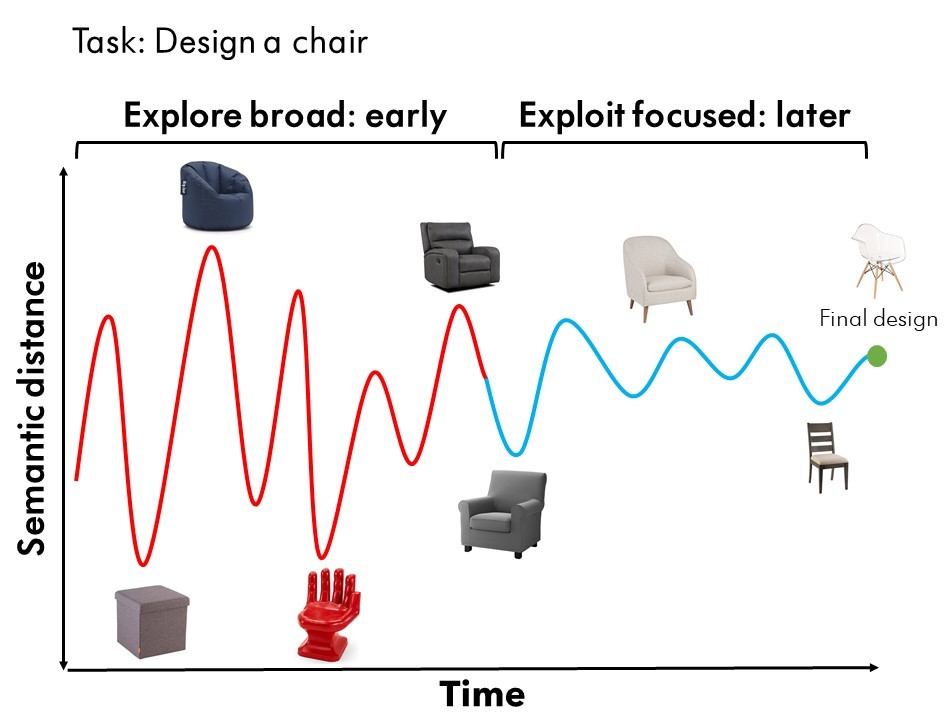
\includegraphics[width=0.9\textwidth]{i_figures/sim-ann.jpg}
  \caption[Creative Annealing: Like simulated annealing, effective creative exploration begins with ``hot’’ broad exploration, bouncing around ideas with high entropy, followed by a ``cool,'' narrow exploitation phase with less entropy.]{Creative Annealing: Like simulated annealing, effective creative exploration begins with ``hot’’ broad exploration, bouncing around ideas with high entropy, followed by a ``cool,'' narrow exploitation phase with less entropy. For example, if the task is to design a chair, one might first start with exploring vastly different types of chairs before narrowing to a more specific type and style of chair.}
  \label{fig:sim-ann}
\end{figure}

\section{The How \& the What of Exploration}

Exploratory thinking comprises both process (how) and content (what) \cite{Kelley2013, kemp2007learning, Newell1962processes, osborn1953applied}. For example, a comic artist might first go through the process of brainstorming potential story ideas for their comic (“how do I get started?”) and then explore various ways of composing their story idea in their comic (“how do I accomplish my goal?”). Once they have their idea, the artist might seek feedback to help them improve (“how do I move forward?”). This dissertation introduces three strategies--incorporated in interactive tools-- that contextually scaffold the process and content of exploratory thinking to help people with the three primary challenges they encounter in creative work (Figure \ref{fig:thesisgrid}). First, abstraction blocks scaffold exploratory process by helping people tangibly explore and communicate alternative ideas in visual creative work. Second, adaptive conceptual guidance, embodied in Sh\”{o}wn, contextually presents examples based on a user’s given progress and activity to improve content exploration. Third, interactive feedback reuse, demonstrated in CritiqueKit, leverages previously-given expert feedback as adaptive suggestions presented alongside interactive structural guidance to also improve content exploration. These strategies and their evaluations demonstrate the potential of structured exploration and adaptive help for amplifying exploratory thinking and overcoming the satisficing bias.

\begin{figure}[b!]
\centering
  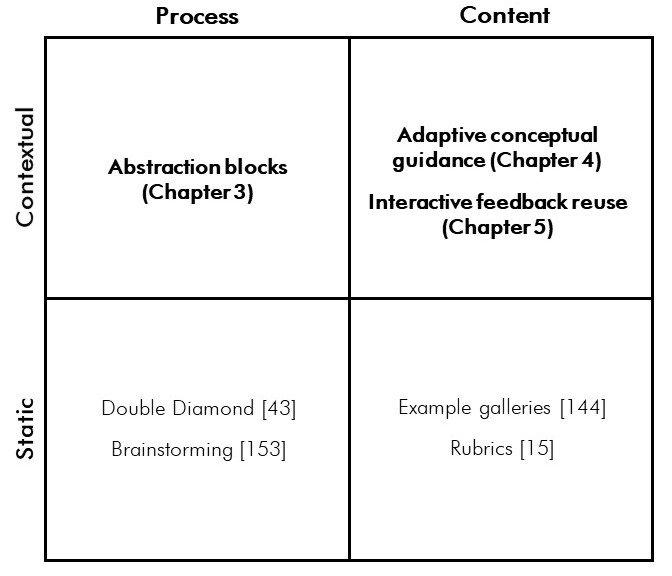
\includegraphics[width=0.8\textwidth]{i_figures/thesis_grid.jpg}
  \caption[The interactive strategies presented in this dissertation (in bold) scaffold both components of exploratory thinking: the process of exploration (how) and the content of exploration (what).]{The interactive strategies presented in this dissertation (in bold) scaffold both components of exploratory thinking: the process of exploration (how) and the content of exploration (what). Bolded entries are the strategies in this dissertation that address contextual and interactive scaffolds for both exploratory process and content. Non-bolded entries are examples of other strategies for scaffolding process and content exploration.}
  \label{fig:thesisgrid}
\end{figure}

% make it clearer in the diagram which ones are mine (i.e. Abstraction Blocks (chapter 3)), and have the reference in the bottom ones.

\section{Structuring Exploration Helps People Get Started in\\ Creative Work}
Common models of design process, such as the Britain Design Council’s Double Diamond (Figure \ref{fig:doublediamond}) \cite{doublediamond} are--for better and for worse--high-level and domain-independent. Empirically, the benefits of such models also remains sparse. Chapter 3 presents a strategy for contextually structuring exploration and evidence of its efficacy.

\subsection{Abstract Blocking Supports Chunking}
Herb Simon’s big contribution to our thinking about expertise is two intertwined ideas: 1) expertise is pattern recognition, and experts know more patterns; and 2) Experts ‘see’ and store patterns in more gestalt, structural terms (what Simon calls ‘chunks’) \cite{Chase1973,Gobet2001,Gobet1998}. Together, this enables experts to see the metaphorical forest for the trees, while novices who lack pattern-recognition chunks, get stymied by the branches.

Chapter 3 hypothesizes that using tangible chunks provides a malleable way for people to explore compositions for visual creative work. I introduce an ‘abstraction blocks’ strategy that embodies this hypothesis (Figure \ref{fig:blocks}). In a collaborative drawing task with six small groups (n=19), groups who used abstraction blocking discussed more high-level concepts and communicated ideas more flexibly than groups who used freeform sketching. 

\section{Contextual Guidance Helps People Accomplish Goals \& Move Forward}
Creative problems are highly contextual: measured success differs depending on the situation and interpretation. For example, Picasso’s abstract drawings are not accurate depictions of the human figure, but are widely regarded as innovative expressions. People need different kinds of help at different times. Assistance that adapts and helps people where they need it most can be powerful for improving creative outcomes. Chapters 4 and 5 utilize adaptive suggestions to provide contextual and individualized help to users at the right moments. 

\subsection{Heuristic Alignment Provides Structure}
While creative work is contextual, there are objective heuristics by which creative work is assessed. These heuristics provide necessary structure for understanding the constraints of a problem space. Rubrics are an example of aligning heuristics between a user and the concept, but they require expertise in developing them and do not provide guidance in how to appropriately address rubric criteria. My insight is that helping align people to conceptual heuristics will improve creative outcomes. Chapter 4 introduces Sh\"{o}wn, which uses heuristic alignment as a way to detect context and provide relevant help for users. In a between-subjects study with novice comic artists, presenting examples based on these heuristics helped people understand why examples were relevant. Chapter 5 applies heuristic alignment as an interactive guidance panel for giving feedback. Two experiments demonstrate that this interactive guidance directs novice reviewers to give more specific, actionable, and justified feedback.

\subsection{Adaptive Suggestions Aid Example Use}
Expert content in the form of video tutorials or expert-produced examples can help guide people in creating something of their own. These examples are useful for providing a point of comparison and inspiration for novices in accomplishing their goals. However, applying the concept behind an example means understanding when the example is most appropriate and relevant. Chapters 4 and 5 explore using adaptive suggestions to present relevant examples and concepts at appropriate moments depending on the user’s task and progress. Chapter 4 introduces the adaptive conceptual guidance strategy and hypothesizes that presenting concepts alongside examples at relevant moments will help novices better understand and apply example concepts. This hypothesis is instantiated in Sh\"{o}wn, a Wizard-of-Oz system for comic drawing. An experiment shows that adaptive conceptual guidance leads to more unique and readable comics compared to showing a library of static examples (Figure \ref{fig:woz}). Chapter 5 presents the CritiqueKit system, which embodies interactive feedback reuse, presenting previously-given expert feedback as adaptive suggestions. Two experiments demonstrate that adaptively reusing and presenting feedback suggestions (Figure \ref{fig:critiquekit_exp2}) improves the quality of critique.

\section{Thesis Statement \& Contributions}
My thesis statement is: 
\begin{quote}
    \textit{Structuring exploration and adaptively presenting help attunes people to a context-appropriate level of detail and leads to better creative outcomes.}
\end{quote}

My dissertation investigates interactive strategies for attuning people towards exploration in the stages of getting started, accomplishing a goal, and moving forward in creative work.

\subsection{Contributions}
Through deployments and controlled studies of these systems, my dissertation contributes both a theoretical understanding of creative cognition and exploratory thinking and practical applications of how these theories are embedded within creativity support tools.
\\
This dissertation contributes the following:

\begin{itemize}
    \item Three strategies that structure exploratory thinking to focus attention on higher-level concepts: abstraction blocks (\textsc{Chapter \ref{chapter:abstraction}}), adaptive conceptual guidance (\textsc{Chapter \ref{chapter:shown}}), and interactive feedback reuse (\textsc{Chapter \ref{chapter:critiquekit}}).
    \item Interactive tools and techniques that embody these strategies and adaptively scaffold exploration within the context of one’s own work.
    \item Empirical evaluations and observations to demonstrate the efficacy of adaptive exploration strategies on improving creative process and content.
    \item Observations of exploration as a pedagogical tool for children and designers.
\end{itemize}
 




